\chapter{O bloco p II: oxigênio, halogênios e gases nobres}\label{ch:b1:p-block-16-18}

O ácido sulfúrico é produzido em maior tonelagem que qualquer outro
produto químico: ele dissolve a rocha fosfática para os fertilizantes,
lixivia minérios de cobre e de urânio, refina petróleo e enche as baterias
de carro, e durante um século a produção de ácido sulfúrico foi uma
medida aproximada da indústria de um país. A maior parte de seu enxofre
vem hoje da purificação do gás natural e do petróleo; uma parte ainda é
carregada à mão para fora de crateras vulcânicas. O enxofre fica no \omterm{def:b1:periodicity:table}{grupo}
16, abaixo do oxigênio; os \omterm{def:b1:p-block-16-18:halogen}{halogênios} do \omterm{def:b1:periodicity:table}{grupo} 17 e os gases nobres do
\omterm{def:b1:periodicity:table}{grupo} 18 completam o \omterm{def:b1:periodicity:table}{bloco} p. Este capítulo acompanha o oxigênio e o
enxofre do elemento ao ácido, classifica os \omterm{def:b1:p-block-16-18:halogen}{halogênios} como \omterm{def:b1:nernst:couple}{oxidantes} por
seus \omterm{def:b1:nernst:electrode-potential}{potenciais padrão} e termina com os compostos que os gases nobres,
supostamente inertes, de fato formam.

\begin{recall}
As \omterm{def:b1:lewis-resonance-vsepr:lewis}{estruturas de Lewis}, os octetos expandidos e as formas VSEPR (\cref{ch:b1:lewis-resonance-vsepr});
os \omterm{def:b1:nernst:electrode-potential}{potenciais padrão} (\cref{ch:b1:nernst}); o \omterm{def:b1:e-ph-diagrams:disproportionation}{desproporcionamento} do
cloro e o \omterm{def:b1:e-ph-diagrams:e-ph-diagram}{diagrama potencial--pH} do cloro
(\cref{ch:b1:e-ph-diagrams}); a catálise (\cref{ch:b1:elementary-steps}).
O Livro 1 (ano 10) agrupou os \omterm{def:b1:p-block-16-18:halogen}{halogênios} e os gases nobres em
famílias.
\end{recall}

\begin{omfigure}
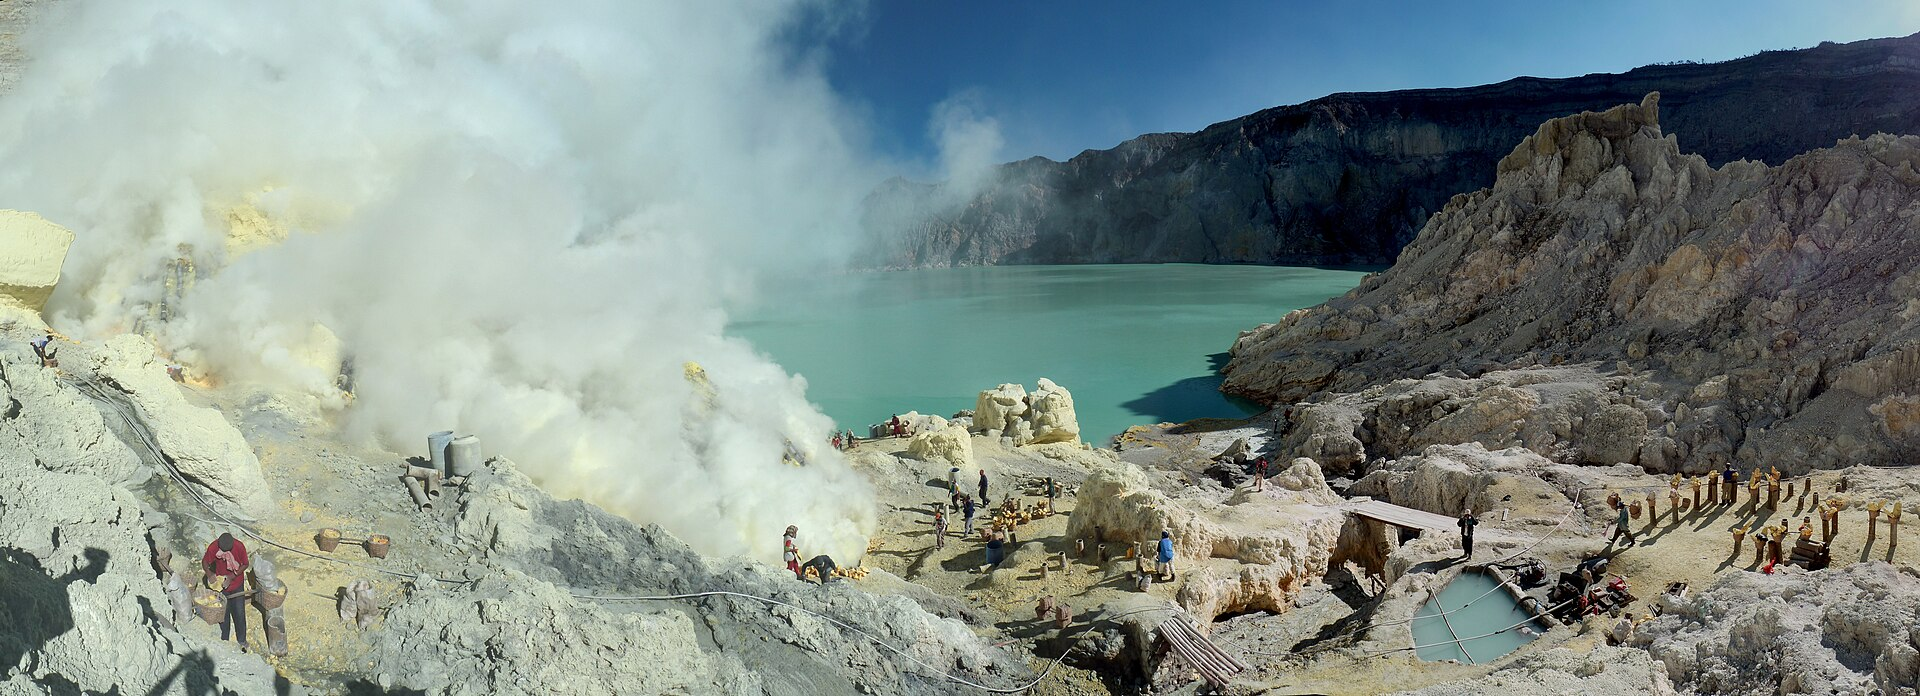
\includegraphics[width=0.78\linewidth]{images/book2/kawah-ijen.jpg}

{\small Extração de enxofre na cratera do vulcão Kawah Ijen, na Indonésia:
os gases vulcânicos condensam enxofre amarelo em torno de tubos, e os
mineiros o carregam para fora em cestos (fotografia de Sémhur, CC BY-SA
4.0, Wikimedia Commons).}
\end{omfigure}

\section{Oxigênio, ozônio e peróxidos}

\begin{definition}[Calcogênios]\label{def:b1:p-block-16-18:chalcogen}
Os \emph{calcogênios}\index{calcogenio@calcogênio} são os elementos do \omterm{def:b1:periodicity:table}{grupo} 16
(O, S, Se, Te, Po), com seis \omterm{def:b1:quantum-numbers:configuration}{elétrons de valência} \textit{ns}$^2$\textit{np}$^4$.
Eles formam compostos com \omterm{def:b1:nernst:oxidation-number}{números de oxidação} de $-$II (óxidos, sulfetos)
a $+$VI (sulfatos), os mais altos apenas do enxofre para baixo.
\end{definition}

O oxigênio existe como dioxigênio \ce{O2} e como ozônio \ce{O3}, uma
molécula angular com duas \omterm{def:b1:lewis-resonance-vsepr:resonance}{estruturas de ressonância} (\cref{ch:b1:lewis-resonance-vsepr}).
O ozônio é um \omterm{def:b1:nernst:couple}{oxidante} mais forte que o dioxigênio: $E^\circ(\ce{O3}/\ce{O2}) = 2.07$~V
contra 1.23~V para \ce{O2}/\ce{H2O}. Na alta atmosfera, ele absorve a luz
ultravioleta; perto do solo, é um poluente. O peróxido de hidrogênio, com
uma ligação \ce{O-O} e o oxigênio em $-$I, é ao mesmo tempo \omterm{def:b1:nernst:couple}{oxidante} e
\omterm{def:b1:nernst:couple}{redutor} e se desproporciona lentamente (\cref{exo:b1:nernst:12}).
% ledger: dfg:O3_g (E0 computed in figdata/bachelor-1/standard-potentials.py)

\begin{example}[Os números de oxidação do oxigênio]
O oxigênio, superado apenas pelo flúor em \omterm{def:b1:periodicity:electronegativity}{eletronegatividade}, está em
$-$II em quase todos os seus compostos: água, óxidos, hidróxidos,
sulfatos. As exceções decorrem da regra segundo a qual os elétrons
compartilhados vão para o parceiro mais eletronegativo e são divididos
igualmente entre átomos idênticos. No peróxido de hidrogênio \ce{H2O2},
H--O--O--H, cada oxigênio fica com os elétrons de sua ligação \ce{O-H},
mas divide o par \ce{O-O}: $-$I. No superóxido de potássio \ce{KO2}, o
íon \ce{O2-} leva uma carga para dois átomos: $-\frac12$ em média. No
difluoreto de oxigênio \ce{OF2}, o flúor ganha as duas ligações e o
oxigênio está em $+$II. Em \ce{O2} e \ce{O3}, ele está em 0. Só o estado
$-$II é estável frente à água; os peróxidos e superóxidos são \omterm{def:b1:nernst:couple}{oxidantes}, e
\ce{OF2} um agente de fluoração.
\end{example}

\section{O enxofre e o ácido sulfúrico}

O enxofre, ao contrário do oxigênio, forma anéis e cadeias de ligações
simples \ce{S-S}: o enxofre comum é formado por anéis \ce{S8}. Ele queima
dando dióxido de enxofre, uma molécula angular (ângulo O--S--O de
\ang{119.5}), que pode ser oxidado ainda a trióxido de enxofre, trigonal
plano. Ambos são \omterm{def:b1:s-block:oxide-character}{óxidos ácidos}: \ce{SO2} dá o ácido sulfuroso
($\mathrm{p}K_a$ 1.77 e 7.22), \ce{SO3} o ácido sulfúrico.
% ledger: geo:SO2.aOSO, dfg:SO2_g, dfg:SO3_g

\begin{proposition}[Etapas do processo de contato]\label{prop:b1:p-block-16-18:contact-steps}
O ácido sulfúrico é produzido a partir do enxofre em quatro etapas:
(1) \ce{S + O2 -> SO2}; (2) \ce{2SO2 + O2 <=> 2SO3}, sobre um \omterm{def:b1:elementary-steps:catalyst}{catalisador}
de óxido de vanádio(V); (3) \ce{SO3 + H2SO4 -> H2S2O7} (óleum), sendo o
trióxido absorvido em ácido concentrado; (4) \ce{H2S2O7 + H2O -> 2H2SO4}.
No total, \ce{2S + 3O2 + 2H2O -> 2H2SO4}.
\end{proposition}

\begin{proof}
Cada etapa está balanceada; somando $2\times(1)$, (2), $2\times(3)$ e
$2\times(4)$, \ce{SO2}, \ce{SO3} e \ce{H2S2O7} se cancelam, e os dois
\ce{H2SO4} consumidos na etapa 3 são regenerados na etapa 4, o que deixa
\ce{2S + 3O2 + 2H2O -> 2H2SO4}. A etapa 2 é termodinamicamente muito
favorável à temperatura ambiente ($K = 10^{24.8}$ a \qty{25}{\celsius}, a
partir das energias de Gibbs de formação), mas extremamente lenta: é o
\omterm{def:b1:elementary-steps:catalyst}{catalisador}, ativo apenas a quente, que a faz andar, e o compromisso entre
velocidade e conversão é estudado no volume do 2.º~ano. O \ce{SO3} não é
absorvido diretamente em água, porque sua reação com o vapor d'água forma
uma névoa fina de gotículas de ácido que atravessa os absorvedores.
\end{proof}
% ledger: dfg:SO2_g, dfg:SO3_g

\begin{omfigure}
\begin{tikzpicture}[font=\small, >={Stealth}, box/.style={draw, rounded corners, fill=omDef!8, align=center, minimum height=1.0cm}]
  \node[box] (b) at (0,0) {queimador de enxofre\\\ce{S + O2 -> SO2}};
  \node[box] (c) at (4.4,0) {conversor, \ce{V2O5}\\leitos catalíticos};
  \node[box] (a) at (8.8,0) {torre de absorção\\\ce{SO3} em \ce{H2SO4}};
  \node[box] (d) at (8.8,-2.2) {diluição\\\ce{H2S2O7 + H2O}};
  \draw[<-, thick] (b.west) -- ++(-0.8,0) node[left] {ar, S};
  \draw[->, thick] (b) -- node[above] {\ce{SO2}} (c);
  \draw[->, thick] (c) -- node[above] {\ce{SO3}} (a);
  \draw[->, thick] (a) -- node[right] {óleum} (d);
  \draw[->, thick] (d.west) -- ++(-1.2,0) node[left] {\ce{H2SO4}};
  \draw[->, thick] (d.east) -- ++(0.6,0) |- node[pos=0.25, right] {parte volta} (a.east);
\end{tikzpicture}

{\small O processo de contato: combustão do enxofre, oxidação catalítica do
\ce{SO2}, absorção do \ce{SO3} em ácido sulfúrico concentrado e diluição
do óleum. Uma parte do ácido é devolvida ao absorvedor.}
\end{omfigure}

\begin{proposition}[Força do ácido sulfúrico]\label{prop:b1:p-block-16-18:sulfuric-strength}
Em água, a primeira acidez do ácido sulfúrico é forte (total), a segunda
fraca: $\mathrm{p}K_a(\ce{HSO4-}/\ce{SO4^2-}) = 1.99$. Uma solução a
\qty{0.010}{mol/L} não está, portanto, nem a pH 1.70 (dois prótons) nem a
2.00 (um), mas entre os dois.
\end{proposition}

\begin{proof}
\ce{H2SO4}, com dois oxigênios sem hidrogênio no enxofre, é um \omterm{def:b1:p-block-13-15:oxoacid}{oxoácido}
mais forte que \ce{H3O+}: nivelado (\cref{ch:b1:predominant-reaction}).
\ce{HSO4-}, já negativo, retém mais seu próton: seu $\mathrm{p}K_a$,
calculado a partir das energias de Gibbs de formação, é 1.99. Para $C = 0.010$:
$[\ce{H3O+}] = C + x$, $[\ce{HSO4-}] = C - x$, $[\ce{SO4^2-}] = x$, com
$x(C + x)/(C - x) = 10^{-1.99}$; resolvendo, $x = \qty{4.2e-3}{mol/L}$ e
$\mathrm{pH} = -\log(0.0142) = 1.85$.
\end{proof}
% ledger: dfg:HSO4-_ao, dfg:SO42-_ao

O ácido sulfúrico concentrado é também um poderoso agente desidratante
(carboniza o açúcar, retirando dele os elementos da água) e, a quente, um
\omterm{def:b1:nernst:couple}{oxidante}. Diluí-lo libera muito calor: o ácido é sempre despejado na
água, nunca o contrário. A maior parte do enxofre do mundo, cerca de 84
milhões de toneladas em 2025, é recuperada do sulfeto de hidrogênio do
gás natural e das correntes de refinaria, e a maior parte termina como
ácido sulfúrico.
% ledger: usgs:S-world-2025

\begin{method}[Balanço de massa ao longo do processo de contato]\label{met:b1:p-block-16-18:contact-balance}
\begin{enumerate}
  \item Use a equação global: um \ce{H2SO4} por átomo de S.
  \item Corrija pela conversão da etapa 2 (a fração de \ce{SO2}
        oxidada) e pelas perdas na absorção.
  \item Para o ar: calcule o \ce{O2} necessário (três meios por S) e
        divida por sua fração no ar.
\end{enumerate}
\end{method}

\begin{example}[Uma fábrica que queima mil toneladas de enxofre por dia]
Uma fábrica queima \qty{1000}{t} de enxofre por dia, converte \qty{99.0}{\percent}
do \ce{SO2} e absorve \qty{99.9}{\percent} do \ce{SO3}. Então
$n(\ce{S}) = \num{1000e6}/32.1 = \qty{3.12e7}{mol}$ e
$n(\ce{H2SO4}) = \num{3.12e7} \times 0.990 \times 0.999
= \qty{3.08e7}{mol}$, isto é, $\num{3.08e7} \times \qty{98.1}{g}
= \qty{3020}{t}$ de ácido por dia. O \qty{1.0}{\percent} não convertido sai
como \ce{SO2}: \qty{3.1e5}{mol}, ou \qty{20}{t} por dia, que precisam ser
removidas do gás de cauda. O dioxigênio necessário é $1.5 \times \num{3.12e7} =
\qty{4.67e7}{mol}$; o ar, com \qty{21}{\percent} de \ce{O2}, é
\qty{2.23e8}{mol}, ou $V = nRT/p = \qty{5.5e6}{m^3}$ por dia a
\qty{25}{\celsius} e \qty{1}{bar}, antes do excesso que a fábrica
realmente insufla.
\end{example}
% ledger: air:O2

\section{Os halogênios}

\begin{definition}[Halogênios]\label{def:b1:p-block-16-18:halogen}
Os \emph{halogênios}\index{halogenio@halogênio} são os elementos do \omterm{def:b1:periodicity:table}{grupo} 17 (F, Cl,
Br, I, At), com sete \omterm{def:b1:quantum-numbers:configuration}{elétrons de valência} \textit{ns}$^2$\textit{np}$^5$.
Eles existem como moléculas diatômicas \ce{X2} e formam íons haleto \ce{X-}.
\end{definition}

\begin{omfigure}
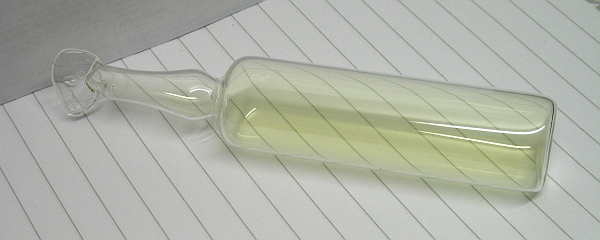
\includegraphics[height=2.9cm]{images/book2/chlorine.jpg}\hspace{0.5em}%
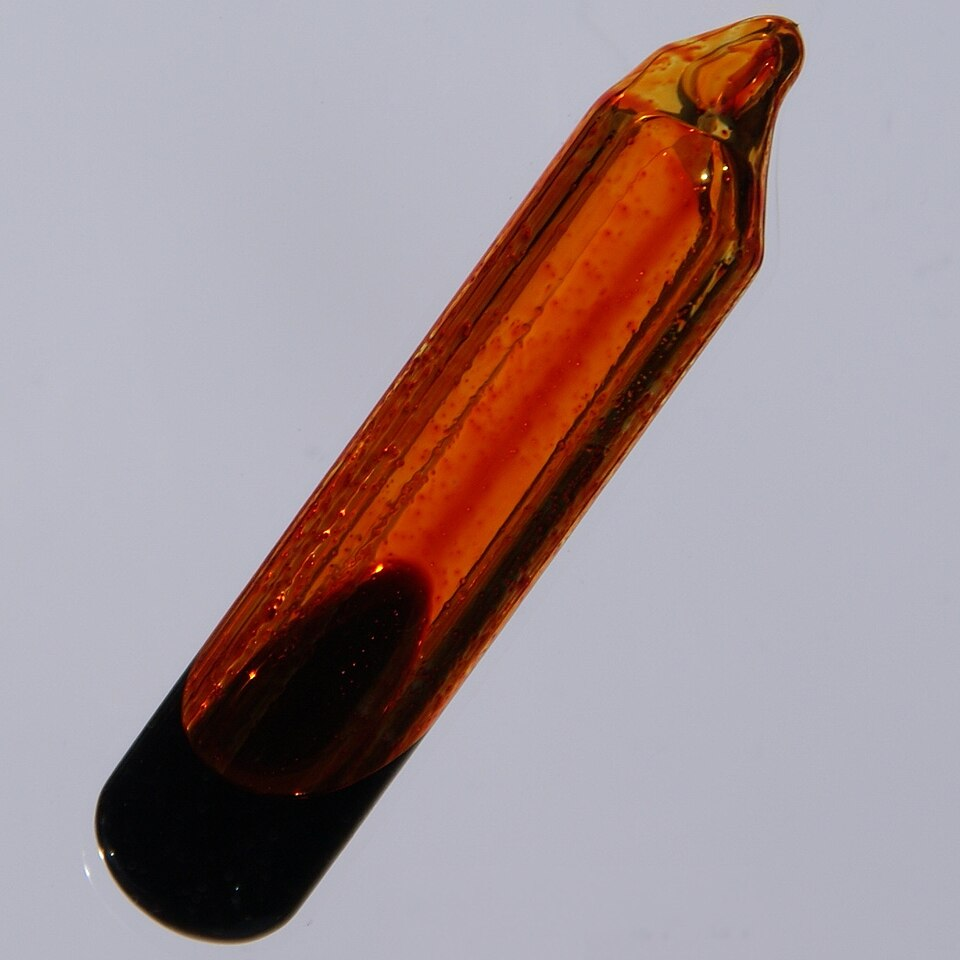
\includegraphics[height=2.9cm]{images/book2/bromine.jpg}\hspace{0.5em}%
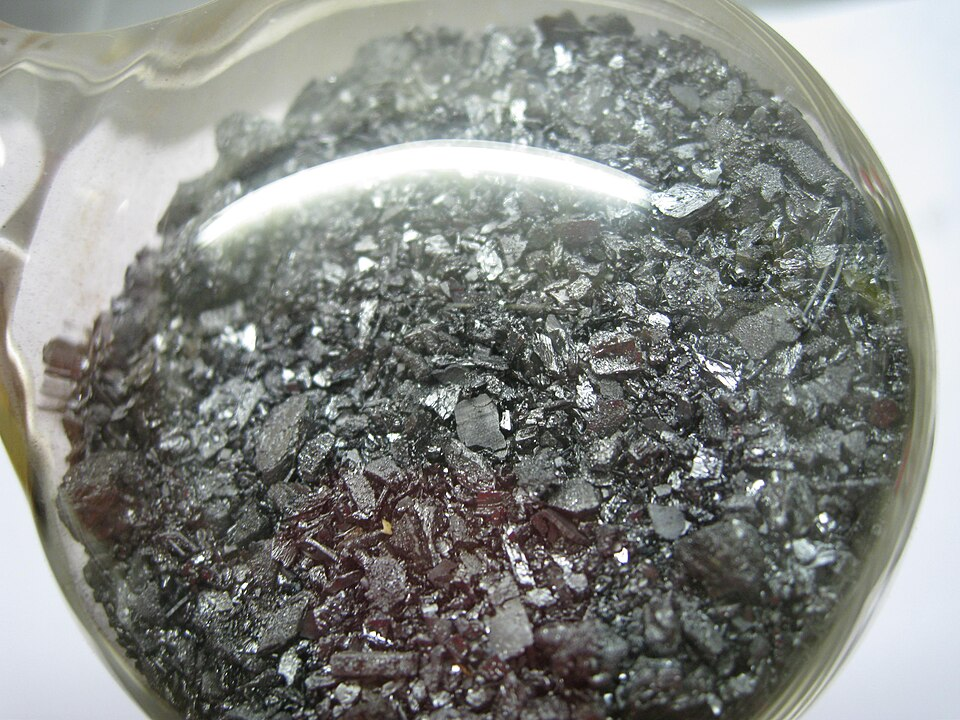
\includegraphics[height=2.9cm]{images/book2/iodine.jpg}

{\small O cloro, um gás amarelo-esverdeado pálido (W. Oelen, CC BY-SA 3.0);
o bromo, um líquido vermelho-escuro de vapor alaranjado (Jurii, CC BY 3.0);
o iodo, \omterm{def:b1:crystals-metals:crystal}{cristais} cinza-escuros de brilho metálico (Dnn87, CC BY 3.0). O
cloro e o bromo estão selados em ampolas de vidro. Todas da Wikimedia Commons.}
\end{omfigure}

\begin{proposition}[Poder oxidante dos halogênios]\label{prop:b1:p-block-16-18:halogen-oxidising-order}
Os \omterm{def:b1:p-block-16-18:halogen}{halogênios} são \omterm{def:b1:nernst:couple}{oxidantes} cuja força diminui ao descer no grupo:
$E^\circ(\ce{F2}/\ce{F-}) = 2.89$~V, \ce{Cl2}/\ce{Cl-} 1.36~V,
\ce{Br2}/\ce{Br-} 1.08~V, \ce{I2}/\ce{I-} 0.53~V. Cada \omterm{def:b1:p-block-16-18:halogen}{halogênio} oxida os
íons haleto situados abaixo dele no grupo.
\end{proposition}

\begin{proof}
Os valores vêm das energias de Gibbs de formação dos íons haleto
(\cref{ch:b1:nernst}). Pela regra do gama, \ce{X2} oxida \ce{Y-} quando o
par \ce{X2}/\ce{X-} fica acima de \ce{Y2}/\ce{Y-}: por exemplo
\ce{Cl2 + 2Br- -> 2Cl- + Br2}, $\log K = 2(1.36 - 1.08)/0.059 = 9.5$.
Descendo no grupo, os átomos crescem, sua afinidade por um elétron extra
e a hidratação dos íons haleto menores diminuem, e o potencial também.
\end{proof}
% ledger: dfg:F-_ao, dfg:Cl-_ao, dfg:Br-_ao, dfg:I-_ao

\begin{omfigure}
\begin{tikzpicture}
\begin{axis}[
  ybar, width=0.62\linewidth, height=5.0cm, ymin=0, ymax=3.3,
  symbolic x coords={F,Cl,Br,I}, xtick=data,
  xticklabels={\ce{F2}/\ce{F-}, \ce{Cl2}/\ce{Cl-}, \ce{Br2}/\ce{Br-}, \ce{I2}/\ce{I-}},
  ylabel={$E^\circ$ (V)}, bar width=16pt, nodes near coords,
  every node near coord/.append style={font=\scriptsize},
  tick label style={font=\small}, label style={font=\small}, enlarge x limits=0.2]
\addplot[fill=omThm!40, draw=omThm] coordinates {(F,2.89) (Cl,1.36) (Br,1.08) (I,0.53)};
\end{axis}
\end{tikzpicture}

{\small \omterm{def:b1:nernst:electrode-potential}{Potenciais padrão} dos pares halogênio--haleto a
\qty{25}{\celsius}, calculados a partir de energias de Gibbs tabeladas: o
poder \omterm{def:b1:nernst:couple}{oxidante} cai de modo regular ao descer no grupo.}
\end{omfigure}

Os haletos de hidrogênio são todos ácidos em água, mas \ce{HF} é fraco
($\mathrm{p}K_a$ 3.16), enquanto \ce{HCl}, \ce{HBr} e \ce{HI} são fortes:
a ligação \ce{H-F} é muito forte e o pequeno íon fluoreto é retido por
\omterm{def:b1:intermolecular-forces-solvents:hbond}{ligações de hidrogênio} fortes. O flúor é o elemento mais eletronegativo e
o \omterm{def:b1:nernst:couple}{oxidante} mais forte da tabela; só é obtido por eletrólise. Os
\omterm{def:b1:p-block-13-15:oxoacid}{oxoácidos} do cloro --- hipocloroso \ce{HClO}, clórico \ce{HClO3},
perclórico \ce{HClO4} --- ficam mais fortes com o número de oxigênios sem
hidrogênio, como todos os \omterm{def:b1:p-block-13-15:oxoacid}{oxoácidos} (\cref{def:b1:p-block-13-15:oxoacid});
sua relação com o cloreto e o cloro foi mapeada no
\cref{ch:b1:e-ph-diagrams}.
% ledger: dfg:HF_ao, dfg:F-_ao

\begin{omfigure}
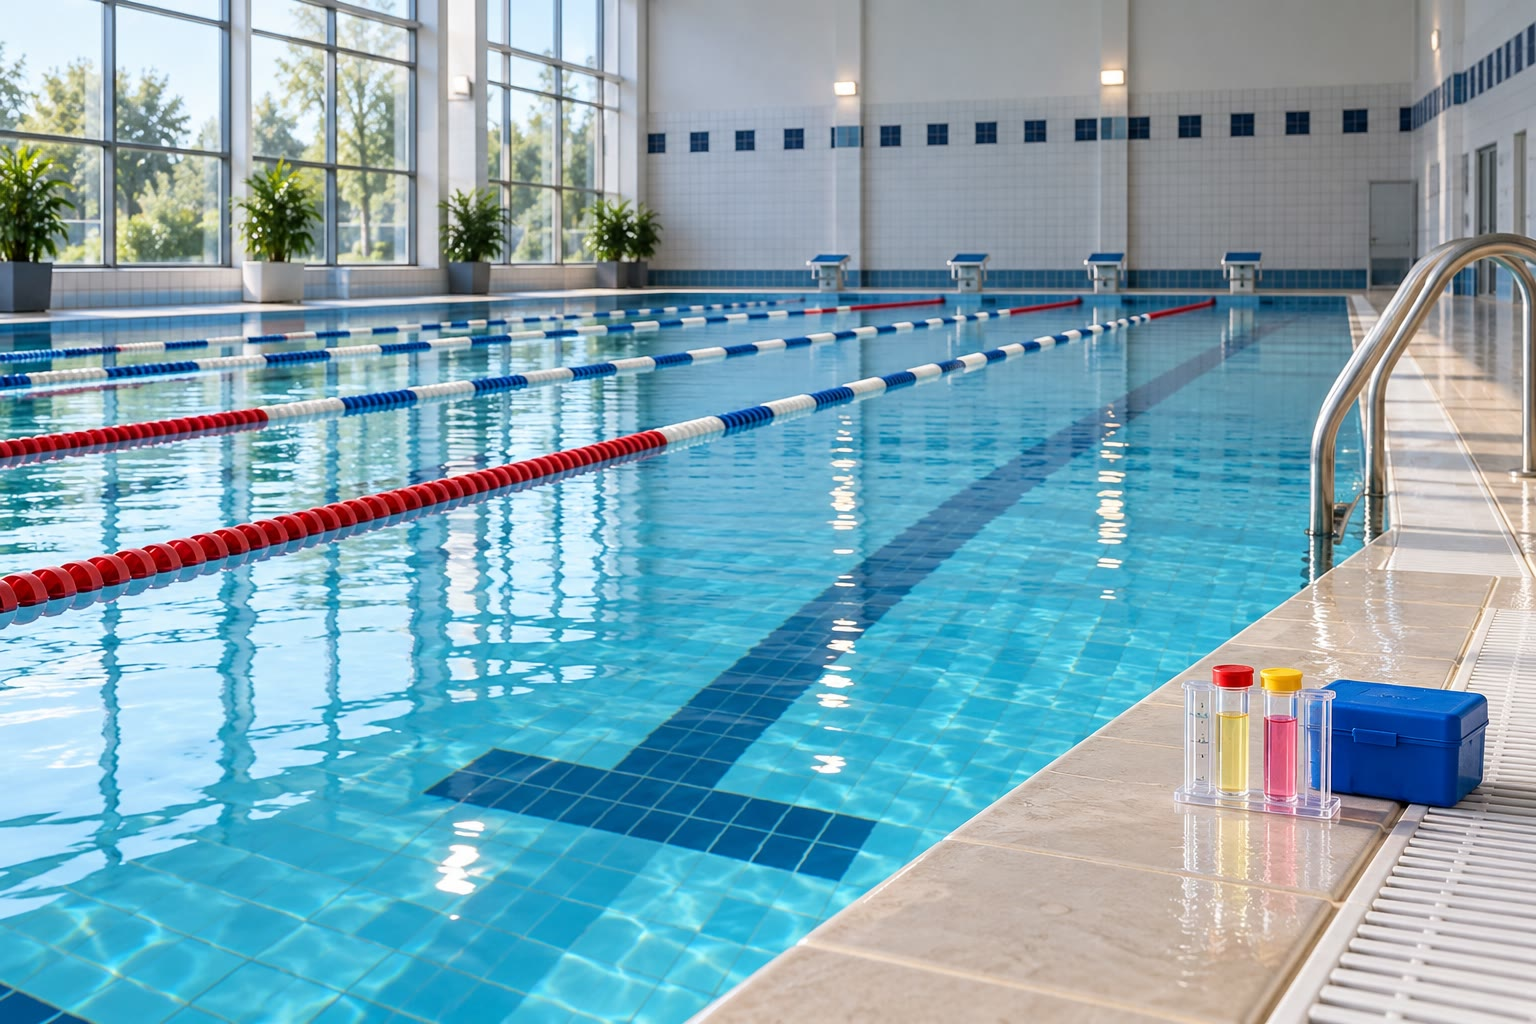
\includegraphics[width=0.55\linewidth]{images/book2/ai/b1-28-swimming-pool.jpg}

{\small Uma piscina pública e seu kit de análise da água: o cloro
dissolvido como ácido hipocloroso é verificado várias vezes por dia.}
\end{omfigure}

\begin{definition}[Compostos inter-halogênios]\label{def:b1:p-block-16-18:interhalogen}
Um \emph{composto inter-halogênio}\index{composto inter-halogenio@composto inter-halogênio} é
um composto de dois \omterm{def:b1:p-block-16-18:halogen}{halogênios} diferentes: \ce{ICl}, \ce{BrF3}, \ce{ClF3},
\ce{IF7}. O \omterm{def:b1:p-block-16-18:halogen}{halogênio} maior e menos eletronegativo é o \omterm{def:b1:complexation:complex}{átomo central}, com
um octeto expandido a partir de \ce{ClF3}.
\end{definition}

\begin{inthelab}[Manipular os halogênios]
O cloro é tóxico e só é preparado em pequenas quantidades, em capela; o
bromo queima a pele e seu vapor ataca os pulmões, e é usado diluído, em
capela, com luvas e óculos, com solução de tiossulfato de sódio à mão
para destruir os derramamentos
(\ce{4Br2 + S2O3^2- + 5H2O -> 8Br- + 2SO4^2- + 10H+}). O iodo é o mais
brando dos três, mas mancha e sublima; é guardado em frasco fechado.
\end{inthelab}

\section{Os gases nobres e seus compostos}

Os gases nobres (He, Ne, Ar, Kr, Xe, Rn) têm camadas de valência
completas e as maiores energias de ionização de seus \omterm{def:b1:periodicity:table}{períodos}
(\cref{ch:b1:periodicity}). Considerados inertes por muito tempo, os mais
pesados, cujos elétrons externos são retidos com menos força, reagem com
os elementos mais eletronegativos: o xenônio dá \ce{XeF2}, \ce{XeF4},
\ce{XeF6} e óxidos. Suas formas seguem as regras VSEPR, com \omterm{def:b1:lewis-resonance-vsepr:lewis}{pares não
ligantes} no xenônio.

\begin{example}[Por que o xenônio, e não o argônio]
As \omterm{def:b1:periodicity:ionisation-energy}{primeiras energias de ionização} dos gases nobres caem ao descer no
grupo: He 24.59, Ne 21.56, Ar 15.76, Kr 14.00, Xe 12.13, Rn 10.75~eV. A do
dioxigênio, \ce{O2 -> O2+ + e-}, é 12.07~eV, quase igual à do xenônio. Um
\omterm{def:b1:nernst:couple}{oxidante} forte o bastante para retirar um elétron de \ce{O2}, dando o
cátion dioxigenila \ce{O2+}, deveria portanto oxidar também o xenônio, mas
não o argônio, que retém seu elétron 3.7~eV mais firmemente. O xenônio de
fato reage com o \omterm{def:b1:nernst:couple}{oxidante} muito forte hexafluoreto de platina \ce{PtF6},
dando um sólido de composição global \ce{XePtF6}, e com o próprio flúor,
que dá os fluoretos de xenônio da tabela abaixo. O radônio, ainda mais
fácil de ionizar, é radioativo demais para que muita química seja feita
com ele.
\end{example}
% ledger: ie:He, ie:Ne, ie:Ar, ie:Kr, ie:Xe, ie:Rn, ie:O2, lit:XePtF6

\begin{omfigure}
\begin{tabular}{llll}
\hline
molécula & pares eletrônicos no \omterm{def:b1:complexation:complex}{átomo central} & forma & ângulo medido \\
\hline
\ce{SO2} & 2 domínios ligantes + 1 \omterm{def:b1:lewis-resonance-vsepr:lewis}{par não ligante} & angular & \ang{119.5} \\
\ce{SF6} & 6 ligantes & octaédrica & \ang{90} \\
\ce{ClF3} & 3 ligantes + 2 \omterm{def:b1:lewis-resonance-vsepr:lewis}{pares não ligantes} & em T & \ang{87.5} \\
\ce{XeF2} & 2 ligantes + 3 \omterm{def:b1:lewis-resonance-vsepr:lewis}{pares não ligantes} & linear & \ang{180} \\
\ce{XeF4} & 4 ligantes + 2 \omterm{def:b1:lewis-resonance-vsepr:lewis}{pares não ligantes} & quadrado-plana & \ang{90} \\
\hline
\end{tabular}

\smallskip
{\small Formas de algumas moléculas do \omterm{def:b1:periodicity:table}{bloco} p com octetos expandidos ou
\omterm{def:b1:lewis-resonance-vsepr:lewis}{pares não ligantes} (ângulos medidos, quando disponíveis). Os \omterm{def:b1:lewis-resonance-vsepr:lewis}{pares não
ligantes} de \ce{XeF2} ocupam as três posições equatoriais de uma
bipirâmide trigonal, o que deixa a molécula linear.}
% ledger: geo:SO2.aOSO, geo:SF6.aFSF, geo:ClF3.aFClF, geo:XeF2.aFXeF
\end{omfigure}

O argônio, quase um por cento do ar, protege materiais reativos nos
laboratórios e na soldagem; o hélio, extraído do gás natural, resfria
ímãs supercondutores, como os dos espectrômetros de RMN (\cref{ch:b1:structure-spectroscopy}).
% ledger: air:Ar

\section{Exercícios}

\begin{exercise}[$\star$]\label{exo:b1:p-block-16-18:1}
Dê o \omterm{def:b1:nernst:oxidation-number}{número de oxidação} do enxofre em \ce{H2S}, \ce{S8}, \ce{SO2},
\ce{SO3^2-}, \ce{SO4^2-}, \ce{S2O3^2-} (médio) e \ce{H2S2O7}.
\end{exercise}

\begin{exercise}[$\star$]\label{exo:b1:p-block-16-18:2}
Quais destas reações ocorrem: cloro com iodeto de potássio; iodo com
brometo de sódio; bromo com cloreto de sódio; cloro com brometo de sódio?
Escreva as que ocorrem.
\end{exercise}

\begin{exercise}[$\star$]\label{exo:b1:p-block-16-18:3}
Desenhe as \omterm{def:b1:lewis-resonance-vsepr:lewis}{estruturas de Lewis} de \ce{SO2}, \ce{SO3} e \ce{O3}, com suas
\omterm{def:b1:lewis-resonance-vsepr:resonance}{estruturas de ressonância}, e dê suas formas.
\end{exercise}

\begin{exercise}[$\star$]\label{exo:b1:p-block-16-18:4}
Escreva as reações de \ce{SO2} e \ce{SO3} com a água e com o hidróxido
de sódio.
\end{exercise}

\begin{exercise}[$\star\star$]\label{exo:b1:p-block-16-18:5}
Calcule o pH do ácido fluorídrico a \qty{0.10}{mol/L} e compare com o
ácido clorídrico na mesma concentração. Explique a diferença.
\end{exercise}

\begin{exercise}[$\star\star$]\label{exo:b1:p-block-16-18:6}
Preveja com o \omterm{def:b1:lewis-resonance-vsepr:vsepr}{modelo VSEPR} as formas de \ce{BrF5}, \ce{IF7} (sete \omterm{def:b1:lewis-resonance-vsepr:lewis}{pares
ligantes}, bipirâmide pentagonal), \ce{ICl4-} e \ce{XeO3}.
\end{exercise}

\begin{exercise}[$\star\star$]\label{exo:b1:p-block-16-18:7}
Calcule a constante de \ce{Cl2 + 2I- -> 2Cl- + I2} e diga por que a água
de cloro azula um papel de amido-iodeto.
\end{exercise}

\begin{exercise}[$\star\star$]\label{exo:b1:p-block-16-18:8}
Mostre que o ozônio pode oxidar os íons iodeto a iodo e escreva a reação
em meio ácido. Por que isso é usado para medir o ozônio?
\end{exercise}

\begin{exercise}[$\star\star$]\label{exo:b1:p-block-16-18:9}
O ácido sulfúrico concentrado carboniza a sacarose, \ce{C12H22O11}.
Escreva a \omterm{def:b1:alcohol-activation:dehydration}{desidratação} a carbono e calcule a massa de carbono obtida a
partir de \qty{10.0}{g} de açúcar.
\end{exercise}

\begin{exercise}[$\star\star\star$]\label{exo:b1:p-block-16-18:10}
Calcule o pH do ácido sulfúrico a \qty{0.10}{mol/L}, levando em conta a
segunda acidez ($\mathrm{p}K_a = 1.99$). Quanto a segunda acidez
acrescenta?
\end{exercise}

\begin{exercise}[$\star\star\star$]\label{exo:b1:p-block-16-18:11}
Usando os potenciais, explique por que o flúor não pode ser preparado
oxidando o fluoreto com nenhum \omterm{def:b1:nernst:couple}{oxidante} químico em água, e por que ele
precisa ser obtido por eletrólise de um fluoreto fundido, e não de uma
solução aquosa.
\end{exercise}

\begin{exercise}[$\star\star\star$]\label{exo:b1:p-block-16-18:12}
O iodo é pouco solúvel em água, mas se dissolve em solução de iodeto de
potássio como íon tri-iodeto \ce{I3-}. Usando as energias de Gibbs de
\ce{I2(aq)} ($\Delta_f G^\circ = \qty{16.40}{kJ/mol}$), \ce{I-} ($-51.57$)
e \ce{I3-} ($-51.4$), calcule a constante de \ce{I2 + I- <=> I3-}.
\end{exercise}

\section{Problema: uma tonelada de enxofre}

\begin{problem}[{Problema de fim de semana --- a combustão do enxofre, a
oxidação catalítica do dióxido de enxofre, a absorção e o óleum, a
segunda acidez do ácido sulfúrico, e a massa de ácido produzida a partir
de uma tonelada de enxofre}]
\label{pb:b1:p-block-16-18:1}
Uma fábrica de ácido sulfúrico queima enxofre recuperado do gás natural.
Massas molares (\unit{g/mol}): S 32.1, \ce{O2} 32.0, \ce{SO2} 64.1, \ce{SO3} 80.1,
\ce{H2SO4} 98.1, \ce{H2O} 18.0; o ar contém \qty{21}{\percent} de
\ce{O2} em volume; $\mathrm{p}K_a(\ce{HSO4-}) = 1.99$; $R =
\qty{8.314}{J/(K.mol)}$.

\medskip
\noindent\textbf{Parte I --- A combustão do enxofre.}
\begin{enumerate}
  \item Dê o \omterm{def:b1:nernst:oxidation-number}{número de oxidação} de S em S, \ce{SO2}, \ce{SO3} e
        \ce{H2SO4}.
  \item Escreva a combustão do enxofre.
  \item Desenhe a \omterm{def:b1:lewis-resonance-vsepr:lewis}{estrutura de Lewis} de \ce{SO2} e preveja sua forma.
  \item Calcule a quantidade de matéria de enxofre em uma tonelada.
  \item Calcule o volume de ar (\qty{25}{\celsius}, \qty{1}{bar}) apenas
        para a combustão.
  \item Por que o gás que sai do queimador é resfriado antes do conversor?
\end{enumerate}

\medskip
\noindent\textbf{Parte II --- A oxidação catalítica.}
\begin{enumerate}[resume]
  \item Escreva a oxidação de \ce{SO2} a \ce{SO3}.
  \item Sua constante a \qty{25}{\celsius} é de cerca de $10^{24.8}$. Por
        que, ainda assim, é preciso um \omterm{def:b1:elementary-steps:catalyst}{catalisador}?
  \item Qual é o papel do óxido de vanádio(V), na linguagem do
        \cref{ch:b1:elementary-steps}?
  \item Desenhe a forma de \ce{SO3}.
  \item Por que se usa ar em excesso?
  \item Que fração do \ce{SO2} se perde se a conversão é de
        \qty{99.7}{\percent}?
\end{enumerate}

\medskip
\noindent\textbf{Parte III --- A absorção.}
\begin{enumerate}[resume]
  \item Escreva a absorção de \ce{SO3} no ácido sulfúrico.
  \item Por que \ce{SO3} não é absorvido diretamente em água?
  \item Escreva a diluição do óleum.
  \item Escreva a equação global do processo.
  \item Calcule a massa de água consumida por tonelada de enxofre.
  \item Por que o ácido deve ser despejado na água e nunca o contrário?
\end{enumerate}

\medskip
\noindent\textbf{Parte IV --- O ácido.}
\begin{enumerate}[resume]
  \item Calcule o pH de uma solução de ácido sulfúrico a \qty{0.050}{mol/L}
        levando em conta a segunda acidez.
  \item Calcule a massa de ácido sulfúrico para um \omterm{def:b1:extent-q-and-k:fractional-extent}{rendimento} global de
        \qty{99.5}{\percent}.
  \item O mundo produziu cerca de \qty{84}{Mt} de enxofre em 2025. Que
        massa de ácido sulfúrico ele daria se fosse todo convertido?
  \item Indique a massa de ácido sulfúrico que se pode obter a partir de
        uma tonelada de enxofre (conversão completa).
\end{enumerate}
\end{problem}
